\section{Problem no.3}
In this last part the aim is to verify the radiating element behavior, starting from the single patch and arriving to the complete array. For the patch antenna we use the one we designed for the second laboratory, that are described in the following image *.
\begin{figure}[H]
	\centering
	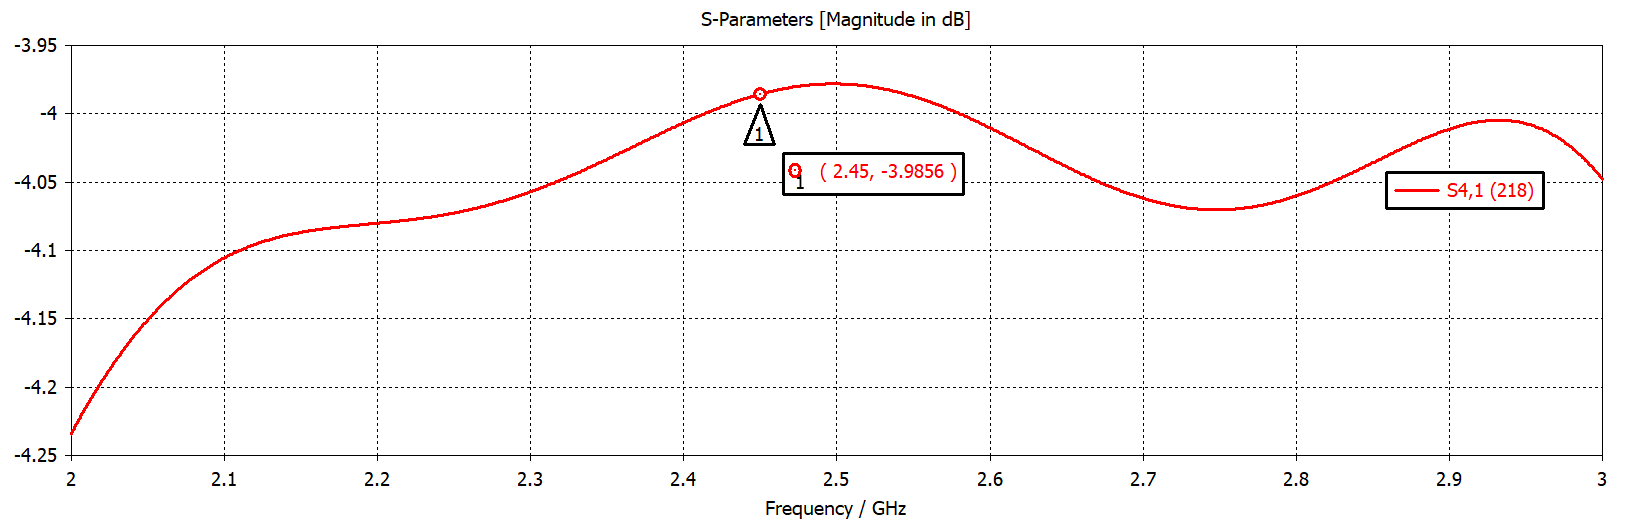
\includegraphics[scale=0.35]{S41Amp.png}
	\caption{S\textsubscript{41} parameter of our BFN}
	\label{S41Amp}
\end{figure}

\paragraph{single antenna} First of all we analyze the single antenna itself, so that we control it resonates at the correct frequency with our feeding. We use a very short line with characteristic impedance close to the patch output one, in order to simulate the effective feeding that will be implemented with the beam forming network. This choice is made also to minimize the contribution due to the mismatching of the load the line, and in fact the length of the microstrip feeding is much less than the guided wavelength at the resonance frequency.
\begin{figure}[H]
	\centering
	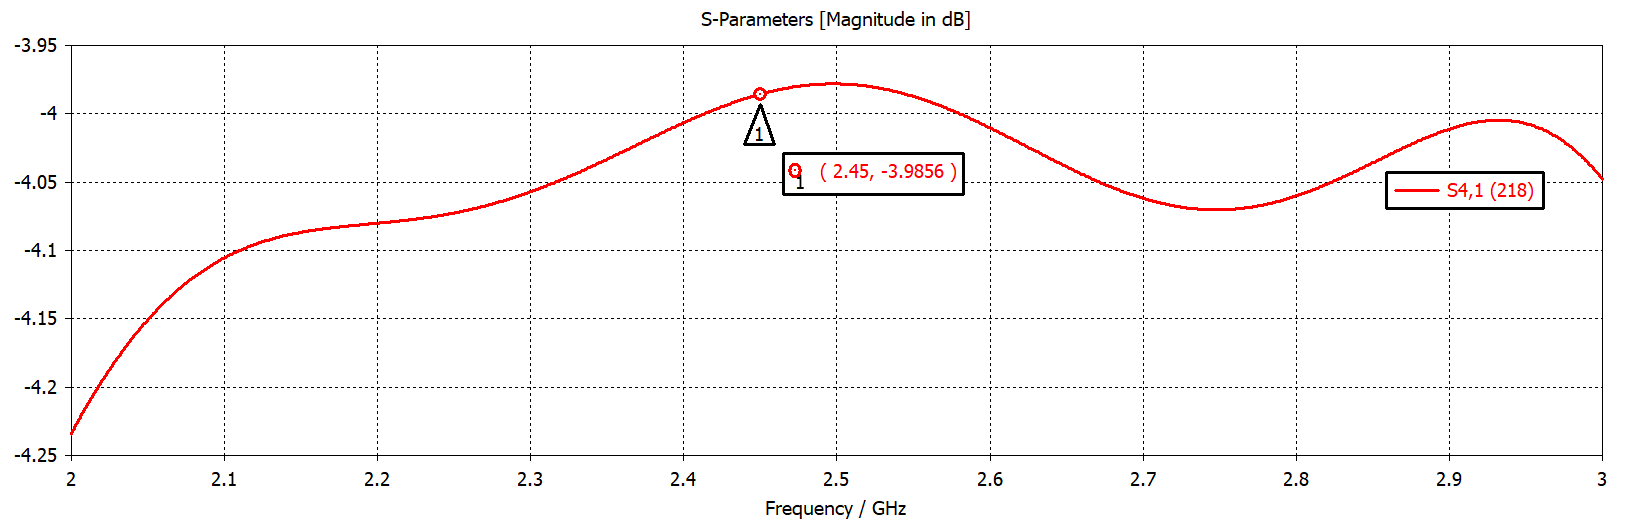
\includegraphics[scale=0.35]{S41Amp.png}
	\caption{S\textsubscript{41} parameter of our BFN}
	\label{S41Amp}
\end{figure}
The initial values shows a behavior not optimal for our situation, and so we have to made a little tuning (not too much because probably the inter element coupling will influence the scattering parameters and it will be required another optimization). *comments*

\paragraph{multiple antennas} Composing the array with those antennas we can have a first simulation of the complete radiating element, and so we can make some considerations. The bigger issue in particular are the resonance frequency, which due to the inter elements coupling (as expected) are deviated from the single antenna case. In particular the resonance frequency results shifted of few hundreds of megahertz upward, movement that we have to take in mind in order to re-design a similar patch antenna complying better with the specifications.
\begin{figure}[H]
	\centering
	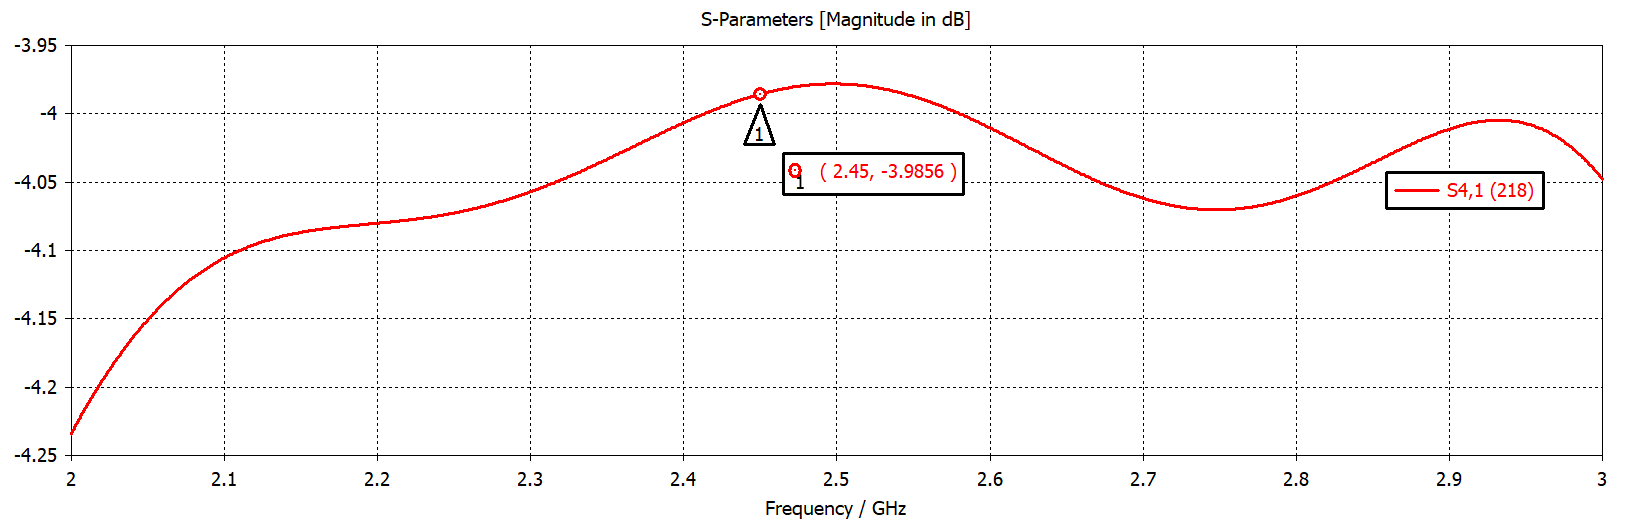
\includegraphics[scale=0.35]{S41Amp.png}
	\caption{S\textsubscript{41} parameter of our BFN}
	\label{S41Amp}
\end{figure}
Simulating the four antennas with their entering ports we have a total number of 16 scattering parameters, which are not so easy to handle in order to find the load seen from the beam forming network point of view and optimize it. Because we use a constant tapering for the antennas feeding we can combine the results of this simulation and find only four scattering parameters describing the reflection coefficient of each port. This way we can also find the relative impedance, so that in our particular case of feeding we can evaluate precisely the active impedance of the antennas. The value founded this way are showed in the figures * and *
\begin{figure}[H]
	\centering
	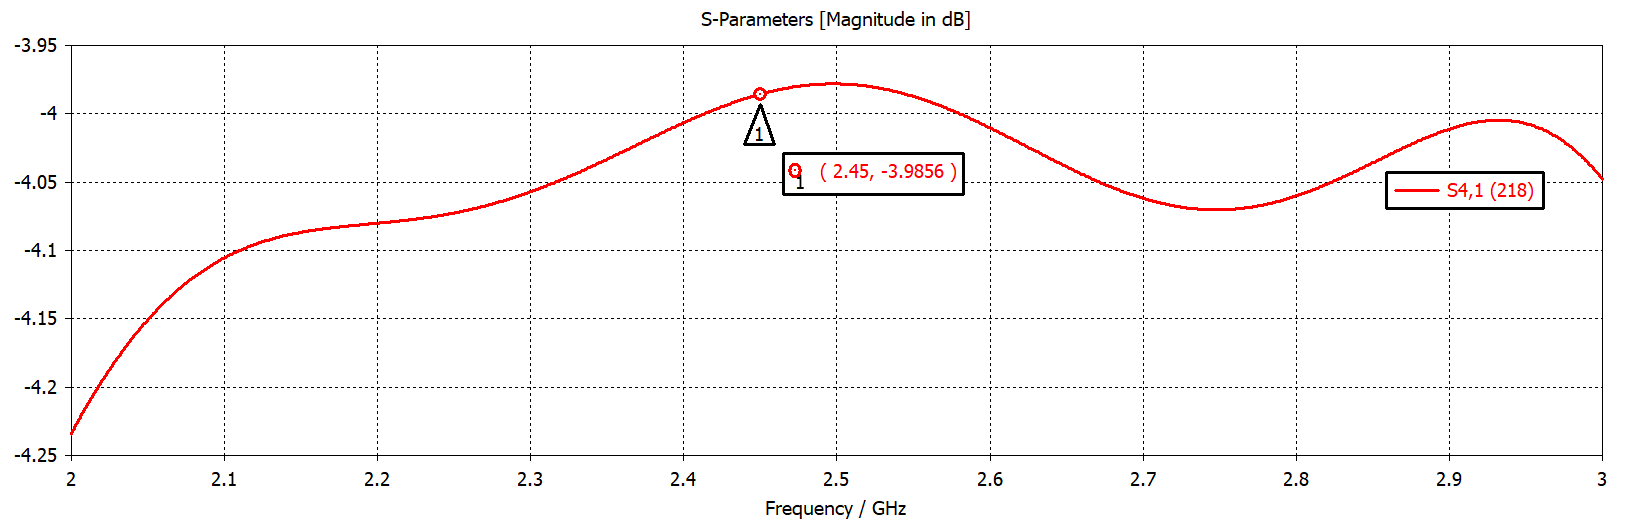
\includegraphics[scale=0.35]{S41Amp.png}
	\caption{S\textsubscript{41} parameter of our BFN}
	\label{S41Amp}
\end{figure}
Cause of the symmetry of the structure we have that the impedance of the external elements slightly differs from the internal one, but as reported in the graph * the difference is negligible.

\paragraph{array factor} The last pass is to consider the radiation pattern, which is first of all evaluated with a far field monitor, and after that is exported and elaborated in Matlab in order to verify the correct behavior of the array factor. For this calculation we need also the far field radiation of the single patch antenna, which must be used as a punctual divider for the array far field (remembering the relation *formula*).
\begin{lstlisting}
% ** preset of all the variables **
alpha=linspace(0,2*pi,10000);
\end{lstlisting}
The result of this calculation is the array factor printed in figure *, which respect all the initial requirements.
\begin{figure}[H]
	\centering
	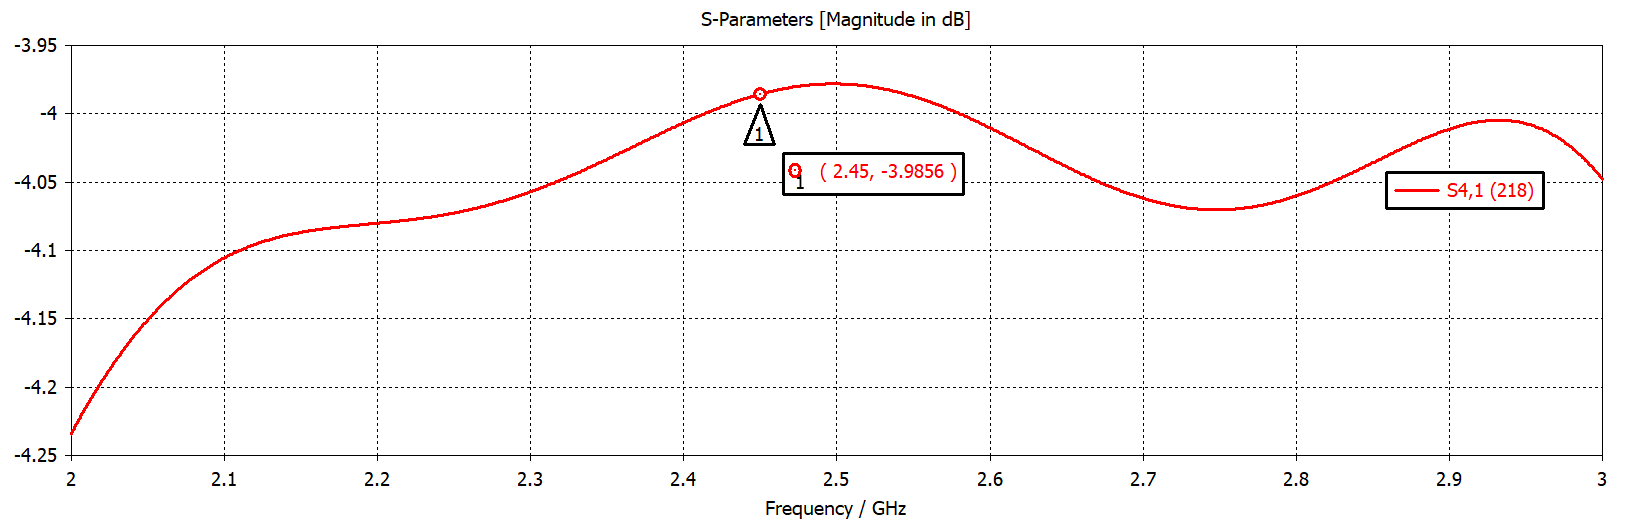
\includegraphics[scale=0.35]{S41Amp.png}
	\caption{S\textsubscript{41} parameter of our BFN}
	\label{S41Amp}
\end{figure}